% fig6_performance_funnel.tex — Run 1 Hit@1 bar chart (TikZ)
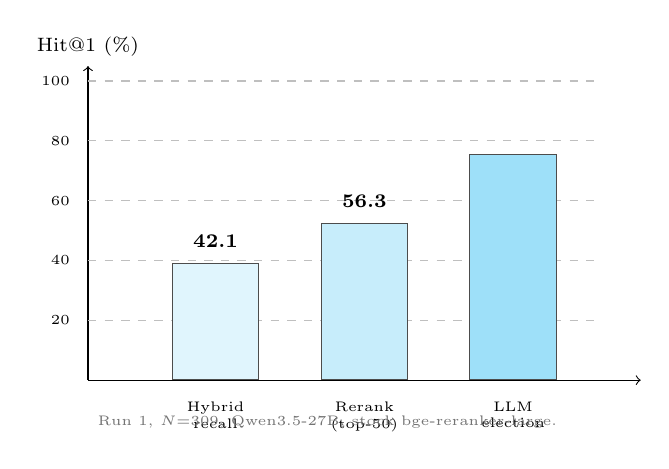
\begin{tikzpicture}[
  x=1.35cm, y=0.038cm,
  font=\small,
  bar/.style={draw=black!70, line width=0.4pt, minimum width=1.1cm, align=center, font=\scriptsize}
]
  \draw[->] (0,0) -- (0,105) node[above, font=\scriptsize] {Hit@1 (\%)};
  \draw[->] (0,0) -- (5.2,0);
  \foreach \y in {20,40,60,80,100} {
    \draw[black!25, dashed] (0,\y) -- (4.8,\y);
    \node[anchor=east, font=\tiny] at (-0.08,\y) {\y};
  }
  \node[bar, anchor=south, fill=cyan!12, minimum height=42.07] (b1) at (1.2,0) {};
  \node[anchor=south, yshift=2pt, font=\scriptsize\bfseries] at (b1.north) {42.1};
  \node[bar, anchor=south, fill=cyan!22, minimum height=56.31] (b2) at (2.6,0) {};
  \node[anchor=south, yshift=2pt, font=\scriptsize\bfseries] at (b2.north) {56.3};
  \node[bar, anchor=south, fill=cyan!38, minimum height=81.23] (b3) at (4.0,0) {};
  \node[anchor=south, yshift=2pt, font=\scriptsize\bfseries, text=white] at (b3.north) {81.2};
  \node[anchor=north, font=\tiny, align=center] at (1.2,-4) {Hybrid\\recall};
  \node[anchor=north, font=\tiny, align=center] at (2.6,-4) {Rerank\\(top-50)};
  \node[anchor=north, font=\tiny, align=center] at (4.0,-4) {LLM\\election};
  \node[anchor=west, font=\tiny, text=black!55] at (0,-14)
    {Run 1, $N{=}309$, Qwen3.5-27B, stock bge-reranker-large.};
\end{tikzpicture}
